\documentclass{article}

\usepackage{polski}
\usepackage[utf8]{inputenc}

\usepackage{fancyhdr} % Required for custom headers
\usepackage{lastpage} % Required to determine the last page for the footer
\usepackage{extramarks} % Required for headers and footers
\usepackage[usenames,dvipsnames]{color} % Required for custom colors
\usepackage{graphicx} % Required to insert images
\usepackage{listings} % Required for insertion of code
\usepackage{courier} % Required for the courier font
\usepackage{lipsum} 
\usepackage{amsfonts}
\usepackage{amsthm}
\usepackage{hyperref}
\usepackage{tikz}
\usepackage{amsmath}
\usepackage{pdfpages}
\usepackage{hyperref}
\usepackage{mathtools}
\usepackage{enumitem}

\usepackage{amsthm}
\usepackage{epigraph}

\DeclareUnicodeCharacter{00A0}{ }

\makeatletter
\newenvironment{chapquote}[2][2em]
  {\setlength{\@tempdima}{#1}%
   \def\chapquote@author{#2}%
   \parshape 1 \@tempdima \dimexpr\textwidth-2\@tempdima\relax%
   \itshape}
  {\par\normalfont\hfill--\ \chapquote@author\hspace*{\@tempdima}\par\bigskip}
\makeatother

\newtheorem{thm}{Twierdzenie}
\newtheorem{remark}{Uwaga}
\newtheorem{lemat}{Lemat}
\newtheorem{wniosek}{Wniosek}
\newtheorem{definicja}{Definicja}
\newtheorem{ciekawostka}{Ciekawostka}
\newtheorem{przyklad}{Przykład}
\newtheorem{fakt}{Fakt}



\newenvironment{prooff}{\paragraph{Dowód:}}{\hfill$\square$}
\newenvironment{rozw}{\paragraph{Rozwiązanie:}}{\hfill}


\usepackage[T1]{fontenc}
\usepackage[scaled=0.84]{beramono}
\usepackage[utf8]{inputenc}
\usepackage[x11names]{xcolor}
\usepackage{listings}
\lstnewenvironment{CPP}
 {\lstset{language=C++,
    basicstyle=\small\ttfamily,
    keywordstyle=\bfseries,
    identifierstyle=\color{red},
    commentstyle=\color{brown},
    stringstyle=\color{blue},
    tabsize=2,
}}{}

% Margins
\topmargin=-0.45in
\evensidemargin=0in
\oddsidemargin=0in
\textwidth=6.0in
\textheight=9.0in
\headsep=0.25in

\linespread{1.1} % Line spacing

% Set up the header and footer
\pagestyle{fancy}
\lhead{\hmwkAuthorName} % Top left header
\rhead{\firstxmark} % Top right header
\lfoot{\lastxmark} % Bottom left footer
\cfoot{} % Bottom center footer
\renewcommand\headrulewidth{0.4pt} % Size of the header rule
\renewcommand\footrulewidth{0.4pt} % Size of the footer rule

\setlength\parindent{0pt} % Removes all indentation from paragraphs
%----------------------------------------------------------------------------------------
%	DOCUMENT STRUCTURE COMMANDS
%	Skip this unless you know what you're doing
%----------------------------------------------------------------------------------------

% Header and footer for when a page split occurs within a problem environment
\newcommand{\enterProblemHeader}[1]{
\nobreak\extramarks{#1}{#1 continued on next page\ldots}\nobreak
\nobreak\extramarks{#1 (continued)}{#1 continued on next page\ldots}\nobreak
}

% Header and footer for when a page split occurs between problem environments
\newcommand{\exitProblemHeader}[1]{
\nobreak\extramarks{#1 (continued)}{#1 continued on next page\ldots}\nobreak
\nobreak\extramarks{#1}{}\nobreak
}

\setcounter{secnumdepth}{0} % Removes default section numbers
\newcounter{homeworkProblemCounter} % Creates a counter to keep track of the number of problems

\newcommand{\homeworkProblemName}{}
\newenvironment{homeworkProblem}[1][Zadanie \arabic{homeworkProblemCounter}]{ % Makes a new environment called homeworkProblem which takes 1 argument (custom name) but the default is "Problem #"
\stepcounter{homeworkProblemCounter} % Increase counter for number of problems
\renewcommand{\homeworkProblemName}{#1} % Assign \homeworkProblemName the name of the problem
\section{\homeworkProblemName} % Make a section in the document with the custom problem count
\enterProblemHeader{\homeworkProblemName} % Header and footer within the environment
}{
\exitProblemHeader{\homeworkProblemName} % Header and footer after the environment
}

\newcommand{\problemAnswer}[1]{ % Defines the problem answer command with the content as the only argument
\noindent\framebox[\columnwidth][c]{\begin{minipage}{0.98\columnwidth}#1\end{minipage}} % Makes the box around the problem answer and puts the content inside
}

\newcommand{\homeworkSectionName}{}
\newenvironment{homeworkSection}[1]{ % New environment for sections within homework problems, takes 1 argument - the name of the section
\renewcommand{\homeworkSectionName}{#1} % Assign \homeworkSectionName to the name of the section from the environment argument
\subsection{\homeworkSectionName} % Make a subsection with the custom name of the subsection
\enterProblemHeader{\homeworkProblemName\ [\homeworkSectionName]} % Header and footer within the environment
}{
\enterProblemHeader{\homeworkProblemName} % Header and footer after the environment
}

\usepackage{listings} % Required for inserting code snippets
\usepackage[usenames,dvipsnames]{color} % Required for specifying custom colors and referring to colors by name

\definecolor{DarkGreen}{rgb}{0.0,0.4,0.0} % Comment color
\definecolor{highlight}{RGB}{255,251,204} % Code highlight color

% Create a command to cleanly insert a snippet with the style above anywhere in the document
\newcommand{\insertcode}[2]{\begin{itemize}\item[]\lstinputlisting[caption=#2,label=#1,style=Style1]{#1}\end{itemize}} % The first argument is the script location/filename and the second is a caption for the listing

%----------------------------------------------------------------------------------------
%	NAME AND CLASS SECTION
%----------------------------------------------------------------------------------------

\newcommand{\hmwkTitle}{Problem palaczy tytoniu} % Assignment title
\newcommand{\hmwkDueDate}{} % Due date
\newcommand{\hmwkClass}{Systemy operacyjne} % Course/class
\newcommand{\hmwkClassTime}{} % Class/lecture time
\newcommand{\hmwkClassInstructor}{} % Teacher/lecturer
\newcommand{\hmwkAuthorName}{Bartosz Bednarczyk - obowiązkowe zadanie z systemów operacyjnych} % Your name

%----------------------------------------------------------------------------------------

\begin{document}
 
\title{Mechanizm bariery dwustopniowej w synchronizacji procesów}
\date{\today}
\author{Bartosz Bednarczyk}
 
\maketitle
 
\subsection*{Motywacja}
 
Podczas zajęć z systemów operacyjnych omówiliśmy wiele metod synchronizacji procesów. W tym sprawozdaniu przedstawię kolejną metodę synchronizacji, zwaną \textbf{barierą}, ale najpierw spójrzmy na poniższe problemy i spróbujmy zauważyć w nich pewne podobieństwo.
 
\begin{itemize}
\item Metoda eliminacji Gaussa. Dzielimy macierz na kilka części i równolegle wykonujemy zadane obliczenia.
\item Problem wyścigu konnych. Wyścig składa się z $N$ rund po jednym okrążeniu. Kolejna runda zaczyna się w momencie, gdy wszystkie konie znajdują się w boksach.
\item Problem ortogonalizacji Grama-Schmidta.
\item Szukanie liczb pierwszych za pomocą sita Eratostenesa.
\end{itemize}
 
\subsection*{Czym jest bariera?}
 
W każdym z powyższych zadań spotykamy następujący problem: każde zadanie dzielmy na podzadania, których wyniki łączymy w jeden na samym końcu. Nie możemy określić wyniku całego zadania bez wcześniejszego połączenia mniejszych podzadań.\\
 
Przejdźmy do abstrakcyjnego pojęcia bariery. Pomyślmy sobie o domu, który ma jedne drzwi wejściowe i jedne wyjściowe. Do takiego domu wchodzi kolejno $N$ gości. Kiedy wejdzie ich już $N$, to zamykamy drzwi wejściowe i otwieramy, początkowo zamknięte, drzwi wyjściowe. Mechanizm bariery jest czymś w rodzaju takiego domu, w którym gośćmi są procesy. Za pomocą tego mechanizmu możemy skutecznie blokować zakończenie podanej operacji do czasu, aż inne procesy zakończą swoje pozadania.
 
\subsection*{Przykładowa implementacja bariery z objaśnieniem}
 
Przykładową implementację bariery umieściłem w pliku ,,bariera.c''. W kodzie mamy dwa semafory o nazwach doorIn oraz doorOut. Początkowo semaforowi doorIn jest przypisana wartość $N$. Oznacza to, że ,,przepuści on przez drzwi'' dokładnie $N$ procesów. Kolejne procesy nie będą wpuszczane do środka. Semafor o nazwie mutex gwarantuje dostęp do licznika procesów. Po jego zdobyciu zwiększmy licznik, a kiedy nie potrzebujemy już danych, to oddajemy je zwalniając mutex. Kiedy $N$-ty proces zwiększa licznik pomiędzy drzwiami, to otwiera on semafor doorOut, który początkowo ustawiony na $0$ (każdy proces się na nim zablokuje). Kiedy pojawia się $N$-ty proces, to otwiera on drzwi tylko dla jednego procesu. Każdy proces przechodzący przez doorOut od razu zamyka drzwi i otwiera je dla kolejnego procesu. W ten sposób procesy przechodzą sznurem przez drzwi wyjściowe. Na samym końcu, kiedy ostatni proces wyszedł drzwiami wyjściowymi, barierę ustawiamy na stan początkowy.


\subsection*{Testy}

Naszą barierę można przetestować próbując zasymulować wyścig konny. Poprawności programu będzie dowodzić to, że nie będzie sytuacji, gdy jeden z koni przebiega metę i dalej biegnie (nie czekając na innych zawodników). Program był uruchamiany wielokrotnie i nie zaobserwowałem by taki przypadek miał miejsce. Poniżej umieszczam przykładową symulację dla pięciu zawodników.

\begin{figure}[h!]
\centering
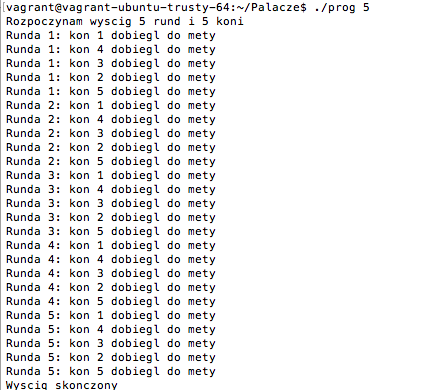
\includegraphics{wyscigscreen}	
\end{figure}

\pagebreak

\subsection*{Dodatek. Kod źródłowy bariery w języku C}

\lstset{inputencoding=utf8}
\lstinputlisting[language=C++]{bariera.c}
\end{document}


\end{document}